\documentclass[12pt]{article}
\usepackage{xeCJK}
\setCJKmainfont{SimSong} 
\usepackage{amsmath, amssymb, bm}
\usepackage{fancyhdr}
\usepackage{graphicx}
\usepackage{listings}
\usepackage{xcolor}
\usepackage{caption}
\usepackage{float}
\usepackage{pythonhighlight}



\definecolor{codegray}{rgb}{0.95,0.95,0.95}
\lstset{
    backgroundcolor=\color{codegray},
    basicstyle=\ttfamily\footnotesize,
    breaklines=true,
    frame=single,
    language=Python,
    keywordstyle=\color{blue},
    commentstyle=\color{gray},
    stringstyle=\color{green!50!black},
    showstringspaces=false
}

\title{Brio–Wu 激波管问题的数值模拟}
\author{231503031 汤轶文}
\date{\today}

\begin{document}

\maketitle

\section{问题背景}

Brio–Wu 激波管问题是磁流体力学(Magnetohydrodynamics, MHD)中的一个标准一维测试问题,用于检验数值方法在求解 MHD 激波、稀疏波、Alfvén 波等复杂波结构时的准确性和稳定性。

\bigskip
该问题模拟的是:一个具有不连续初始条件的磁流体系统在时间演化中形成多个典型的 MHD 波,包括快激波、慢激波、稀疏波、接触间断与 Alfvén 波。

\section{理想 MHD 方程与理论推导}

在一维情况下,理想 MHD 的守恒形式为:

\[
\frac{\partial \bm{U}}{\partial t} + \frac{\partial \bm{F}(\bm{U})}{\partial x} = 0
\]

其中守恒变量为:

\[
\bm{U} =
\begin{bmatrix}
\rho \\
\rho v_x \\
\rho v_y \\
\rho v_z \\
B_y \\
B_z \\
E
\end{bmatrix}, \quad
\mbox{总能量为:} \quad
E = \frac{p}{\gamma - 1} + \frac{1}{2} \rho v^2 + \frac{1}{2} B^2
\]

通量函数为:

\[
\bm{F}(\bm{U}) =
\begin{bmatrix}
\rho v_x \\
\rho v_x^2 + p_t - B_x^2 \\
\rho v_x v_y - B_x B_y \\
\rho v_x v_z - B_x B_z \\
v_x B_y - v_y B_x \\
v_x B_z - v_z B_x \\
(E + p_t) v_x - B_x(\bm{v} \cdot \bm{B})
\end{bmatrix}
\]

其中总压为:
\[
p_t = p + \frac{1}{2} B^2
\]

\subsection*{初始条件(Brio–Wu)}

\begin{itemize}
    \item 左侧 ($x < 0.5$):$\rho = 1.0,\quad p = 1.0,\quad v = 0,\quad B_y = 1.0$
    \item 右侧 ($x > 0.5$):$\rho = 0.125,\quad p = 0.1,\quad v = 0,\quad B_y = -1.0$
    \item 两侧共用:$B_x = 0.75,\quad B_z = 0$
\end{itemize}

系统将在时间演化中形成一系列 MHD 波结构。

\section{数值方法}

\subsection*{时间推进(Euler 显式)}
守恒格式的一阶时间推进方法为:

\[
\bm{U}_i^{n+1} = \bm{U}_i^n - \frac{\Delta t}{\Delta x} \left( \bm{F}_{i+1/2} - \bm{F}_{i-1/2} \right)
\]

\subsection*{数值通量(HLL 方法)}
为简化求解 Riemann 问题,我们采用 HLL 数值通量:

\[
\bm{F}_{\text{HLL}} =
\begin{cases}
\bm{F}_L, & S_L > 0 \\
\bm{F}_R, & S_R < 0 \\
\frac{S_R \bm{F}_L - S_L \bm{F}_R + S_L S_R (\bm{U}_R - \bm{U}_L)}{S_R - S_L}, & \text{otherwise}
\end{cases}
\]

波速估计:
\[
S_L = \min(v_L - a_L,\; v_R - a_R), \quad
S_R = \max(v_L + a_L,\; v_R + a_R)
\]

\section{Python 实现}

程序用 Python 编写,基于有限体积法、HLL 通量和 Euler 显式时间推进。

\subsection*{主要代码结构}

\begin{itemize}
    \item \texttt{initial\_conditions}:设置初值
    \item \texttt{compute\_flux}:计算理想 MHD 通量
    \item \texttt{hll\_flux}:实现 HLL 通量
    \item \texttt{evolve}:时间推进核心函数
    \item \texttt{main}:时间循环与可视化
\end{itemize}

\subsection*{关键代码片段}

\begin{lstlisting}[language=Python, caption=HLL 数值通量计算]
def hll_flux(UL, UR, Bx):
    flux_L = compute_flux(UL, Bx)
    flux_R = compute_flux(UR, Bx)

    rhoL, mxL, *_ = UL
    rhoR, mxR, *_ = UR
    vxL = mxL / rhoL
    vxR = mxR / rhoR
    aL = np.sqrt(gamma * compute_pressure(UL, Bx) / rhoL)
    aR = np.sqrt(gamma * compute_pressure(UR, Bx) / rhoR)

    SL = np.minimum(vxL - aL, vxR - aR)
    SR = np.maximum(vxL + aL, vxR + aR)

    flux = np.where(SL > 0, flux_L,
             np.where(SR < 0, flux_R,
             (SR * flux_L - SL * flux_R + SL * SR * (UR - UL)) / (SR - SL)))
    return flux
\end{lstlisting}

完整代码请见附录。

\section{模拟结果与分析}

在模拟终止时(例如 $t = 0.1, 0.2$),我们对密度 $\rho$、速度 $v_x$ 和磁场 $B_y$ 进行可视化。

\begin{figure}[H]
    \centering
    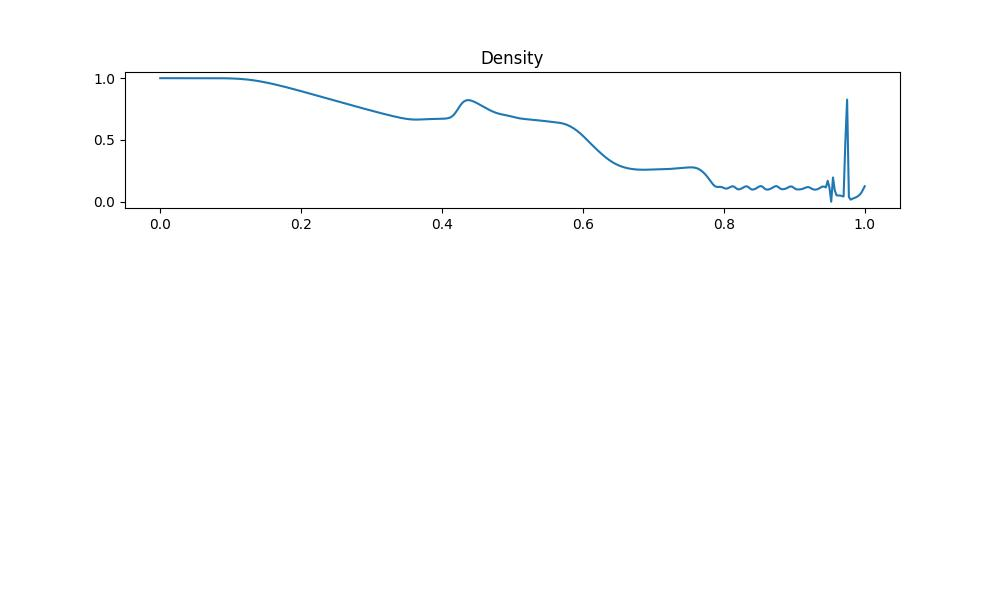
\includegraphics[width=0.85\textwidth]{density.jpg}
    \caption{密度 $\rho$ 的演化}
\end{figure}

\begin{figure}[H]
    \centering
    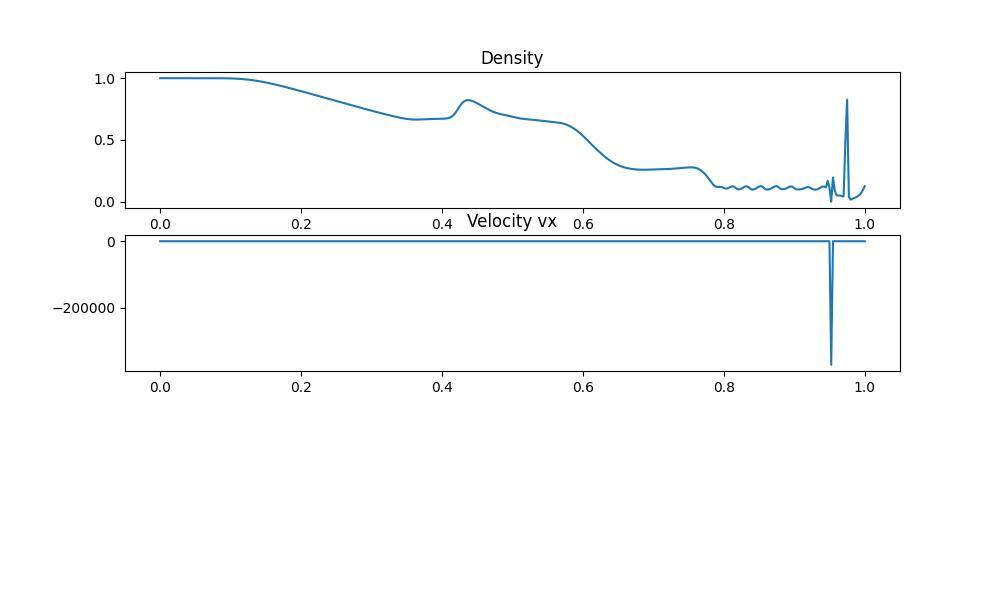
\includegraphics[width=0.85\textwidth]{velocity.jpg}
    \caption{速度 $v_x$ 的演化}
\end{figure}

\begin{figure}[H]
    \centering
    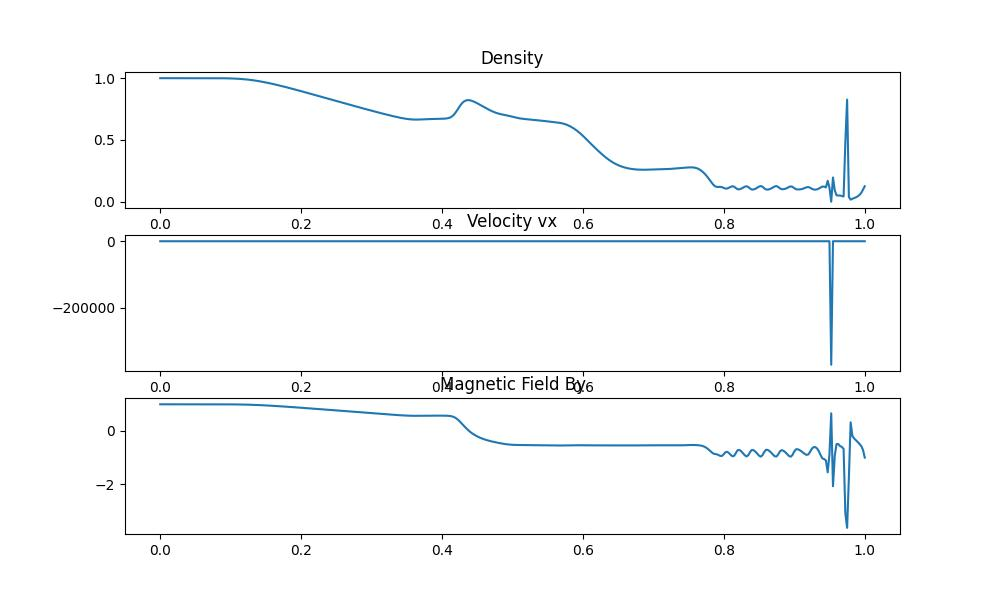
\includegraphics[width=0.85\textwidth]{magnetic_field.jpg}
    \caption{磁场 $B_y$ 的演化}
\end{figure}

\subsection*{物理现象识别}
从图中我们可清晰识别出:

\begin{itemize}
    \item 快激波和慢激波造成的密度和速度突变
    \item 中间位置的接触间断
    \item $B_y$ 中明显的 Alfvén 波结构(尖锐拐角)
\end{itemize}

这些特征与理论分析一致,说明数值模拟成功复现了 MHD 典型波结构。

\section{结论}

本实验通过数值求解 Brio–Wu 激波管问题,成功模拟出理想 MHD 中典型的波动行为,包括慢/快磁声波、Alfvén 波和接触间断。所用的 HLL 数值通量和 Euler 显式推进具有良好的稳定性和结构保持能力,为后续更复杂二维/高阶 MHD 模拟打下基础。

\section{附录-完整代码}
\begin{python}
    import numpy as np
import matplotlib.pyplot as plt

N = 400                  
x = np.linspace(0, 1, N) 
dx = x[1] - x[0]
gamma = 2.0              
CFL = 0.4
t_end = 0.2

def initial_conditions():
    rho = np.where(x < 0.5, 1.0, 0.125)
    vx  = np.where(x < 0.5, 0.0, 0.0)
    vy  = np.where(x < 0.5, 0.0, 0.0)
    vz  = np.where(x < 0.5, 0.0, 0.0)
    By  = np.where(x < 0.5, 1.0, -1.0)
    Bz  = np.where(x < 0.5, 0.0, 0.0)
    Bx  = 0.75
    p   = np.where(x < 0.5, 1.0, 0.1)

    v2 = vx**2 + vy**2 + vz**2
    B2 = Bx**2 + By**2 + Bz**2
    E = p / (gamma - 1) + 0.5 * rho * v2 + 0.5 * B2

    U = np.array([rho, rho*vx, rho*vy, rho*vz, By, Bz, E])  # shape: (7, N)
    return U, Bx

def compute_flux(U, Bx):
    rho, mx, my, mz, By, Bz, E = U
    vx = mx / rho
    vy = my / rho
    vz = mz / rho

    p_gas = (gamma - 1) * (E - 0.5 * rho * (vx**2 + vy**2 + vz**2) - 0.5 * (Bx**2 + By**2 + Bz**2))
    ptot = p_gas + 0.5 * (Bx**2 + By**2 + Bz**2)


    flux = np.array([
        mx,
        mx * vx + ptot - Bx**2,
        my * vx - Bx * By,
        mz * vx - Bx * Bz,
        By * vx - vy * Bx,
        Bz * vx - vz * Bx,
        (E + ptot) * vx - Bx * (vx * Bx + vy * By + vz * Bz)
    ])
    return flux

def hll_flux(UL, UR, Bx):

    flux_L = compute_flux(UL, Bx)
    flux_R = compute_flux(UR, Bx)

    rhoL, mxL, *_ = UL
    rhoR, mxR, *_ = UR
    vxL = mxL / rhoL
    vxR = mxR / rhoR
    aL = np.sqrt(gamma * (compute_pressure(UL, Bx)) / rhoL)
    aR = np.sqrt(gamma * (compute_pressure(UR, Bx)) / rhoR)

    SL = np.minimum(vxL - aL, vxR - aR)
    SR = np.maximum(vxL + aL, vxR + aR)

    # HLL flux
    flux = np.where(SL > 0, flux_L, np.where(SR < 0, flux_R, (SR * flux_L - SL * flux_R + SL * SR * (UR - UL)) / (SR - SL)))
    return flux

def compute_pressure(U, Bx):
    rho, mx, my, mz, By, Bz, E = U
    vx = mx / rho
    vy = my / rho
    vz = mz / rho
    kinetic = 0.5 * rho * (vx**2 + vy**2 + vz**2)
    magnetic = 0.5 * (Bx**2 + By**2 + Bz**2)
    p = (gamma - 1) * (E - kinetic - magnetic)
    return np.clip(p, 1e-10, np.inf)

def timestep(U, Bx):
    rho, mx, *_ = U
    vx = mx / rho
    a = np.sqrt(gamma * compute_pressure(U, Bx) / rho)
    max_speed = np.max(np.abs(vx) + a)
    dt = CFL * dx / max_speed
    return dt

def evolve(U, Bx, dt):
    UL = U[:, :-1]
    UR = U[:, 1:]
    flux = hll_flux(UL, UR, Bx)

    U_new = U.copy()
    U_new[:, 1:-1] -= dt / dx * (flux[:, 1:] - flux[:, :-1])
    return U_new

def main():
    U, Bx = initial_conditions()
    t = 0.0
    while t < t_end:
        dt = timestep(U, Bx)
        if t + dt > t_end:
            dt = t_end - t
        U = evolve(U, Bx, dt)
        t += dt
        print(f"t = {t:.4f}", end='\r')


    rho = U[0]
    vx = U[1] / U[0]
    By = U[4]


    plt.figure(figsize=(10, 6))

    plt.subplot(3, 1, 1)
    plt.plot(x, rho)
    plt.title('Density')
    plt.savefig('density.jpg') 

    plt.subplot(3, 1, 2)
    plt.plot(x, vx)
    plt.title('Velocity vx')
    plt.savefig('velocity.jpg') 

    plt.subplot(3, 1, 3)
    plt.plot(x, By)
    plt.title('Magnetic Field By')
    plt.savefig('magnetic_field.jpg')

    plt.tight_layout()
    plt.close() 
    print("Done!")
if __name__ == '__main__':
    main()

\end{python}
\end{document}